\section{SoDA -- Solid for Data Altruism}
\label{sec:soda}

This Section features an architecture designed to enable data altruism as a service, utilising the Solid protocol and ODRL policies to facilitate the sharing of personal data for altruistic purposes in a manner that respects data protection principles.
The policies are articulated using OAC and the DGAterms concepts related to data altruism.
Furthermore, we introduce the Solid Data Altruism application, SoDA, which allows (a) individuals to create policies for sharing their personal data for altruistic purposes, (b) data users to request access to datasets for altruistic purposes, and (c) data altruism organisations to manage metadata concerning available datasets.

\subsection{Solid architecture for data altruism}
\label{sec:architecture_soda}

The diagram presented in Figure~\ref{fig:soda_architecture} provides a broad summary of an architecture designed to implement data altruism as a service through the usage of the Solid protocol, with the central component being a Solid for Data Altruism application, known as SoDA.
The objective of this architecture is to start a proof of concept decentralised ecosystem for data altruism, emphasising the capability of data subjects to share personal data and data users to discover available datasets suitable for altruistic purposes, in line with data protection principles in the EU as the information disclosed about each dataset is limited to its data type and the intended purpose for its utilisation.

\begin{figure}[ht]
  \centering
  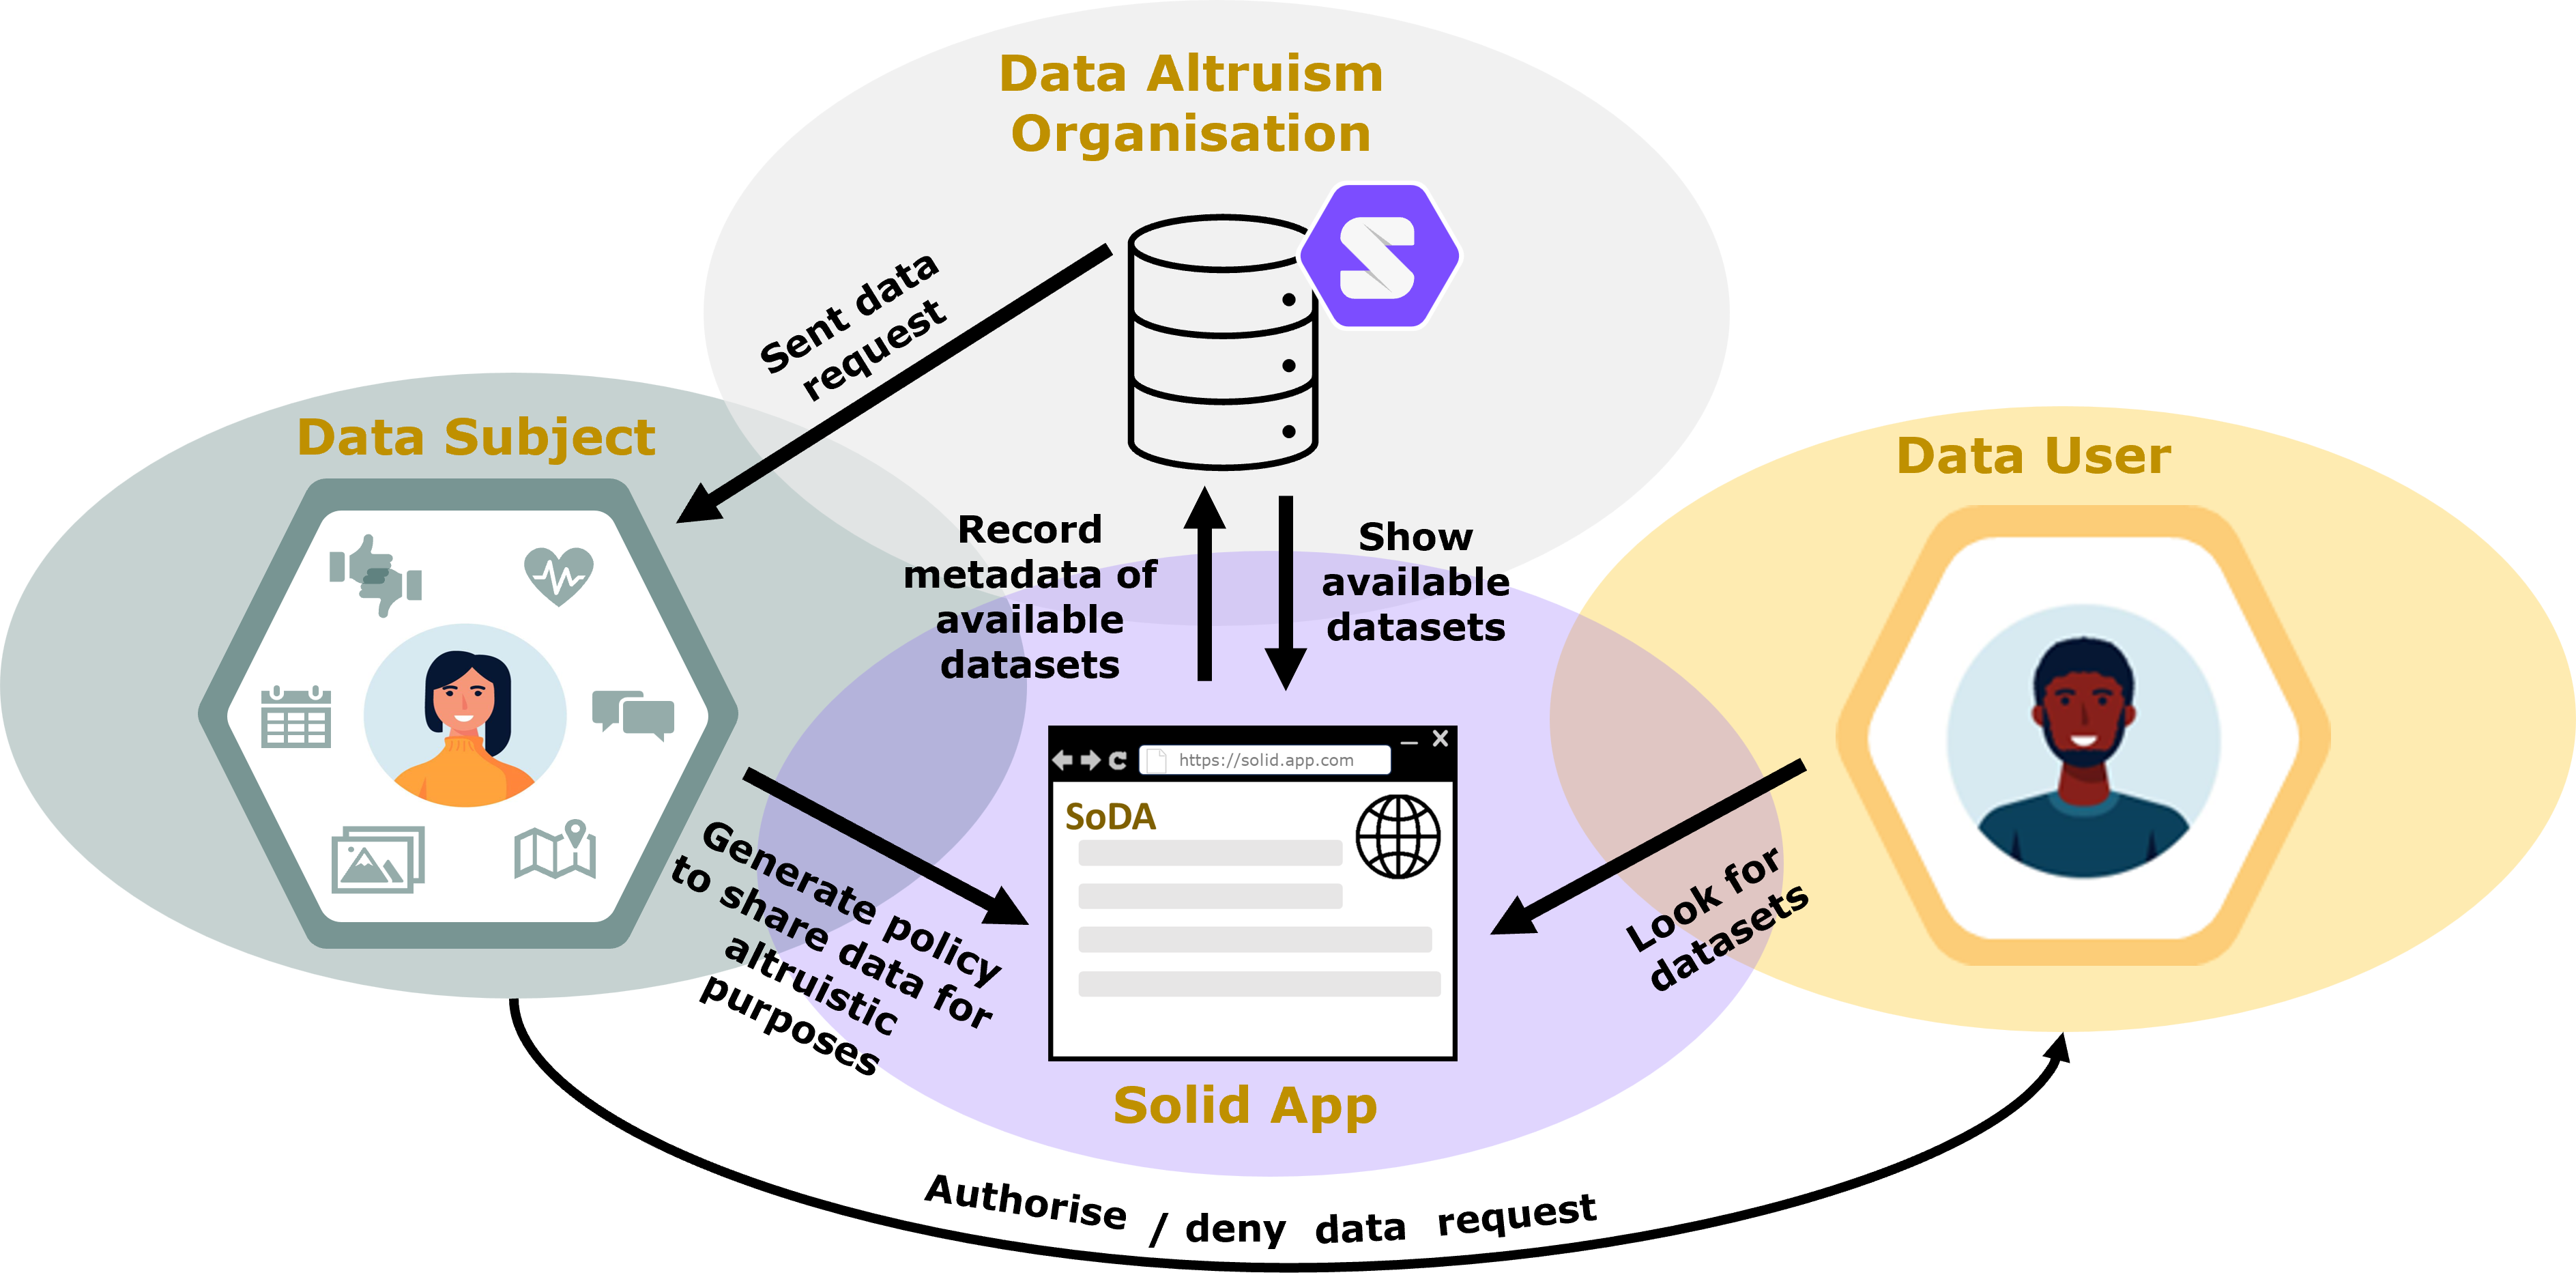
\includegraphics[width=\linewidth]{figures/chapter-7/architecture.png}
  \caption{High-level diagram speifying an architecture to implement data altruism as a service using Solid and SoDA, a Solid application to edit policies/search for data for altruistic purposes, adapted from \cite{esteves_towards_2023}.}
  \label{fig:soda_architecture}
\end{figure}

As previously described, within a Solid-based architecture, users are recognised through a WebID and utilise Solid Pods to either store data or request access to stored data, adhering to the specifications outlined in the Solid protocol.
When personal data resides within Pods, GDPR and DGA requirements come into effect, with individuals who store their personal data in Pods being categorised as `data subjects'.
Additionally, both data subjects and data users administer data access via Solid applications.
In this setting, the SoDA application is introduced to:

\begin{enumerate}
    \item [(a)] empower data subjects to create policies for sharing their personal data with altruistic intent;
    \item [(b)] enable users to seek access to datasets based on their data type and intended purpose for usage; and
    \item [(c)] facilitate organisations in offering data altruism services by maintaining metadata about accessible datasets within their own Solid Pod, without the necessity of storing the data themselves, aligning with Solid's decentralised principles.
\end{enumerate}
